%!TEX TS-program = xelatex
%!TEX encoding = UTF-8 Unicode

\documentclass[a4paper,11pt,french]{article}

%Import des packages utilisés pour le document
\usepackage[latin1]{inputenc}
\usepackage[french]{babel}
\usepackage{chngpage}
\usepackage[colorlinks=true,linkcolor=black,urlcolor=blue]{hyperref}
\usepackage{graphicx, amssymb, color, listings}
\usepackage{fontspec,xltxtra,xunicode,color}
\usepackage{tabularx, longtable}
\usepackage[table]{xcolor}
\usepackage{fancyhdr}
\usepackage{tikz}
\usetikzlibrary{shapes}
\usepackage{lastpage}

\definecolor{gris}{rgb}{0.95, 0.95, 0.95}

%Redéfinition des marges
\addtolength{\hoffset}{-2cm}
\addtolength{\textwidth}{4cm}
\addtolength{\topmargin}{-2cm}
\addtolength{\textheight}{1cm}
\addtolength{\headsep}{0.8cm} 
\addtolength{\footskip}{1cm}


%Import page de garde et structures pour la gestion de projet
\usepackage{res/structures} 

%Variables
\def\matiere{Conduite de Projet}
\def\filiere{Master 2 SSI}
\def\projectDesc{Smart Social Network}
\def\projectName{\emph{SSN}~}
\def\completeName{\projectDesc ~- \projectName}
\def\docType{Plan de développement}
\def\docDate{\today}
\def\version{0.1}
\def\author{Florian \textsc{Guilbert}}
\def\checked{}
\def\approved{}


% -- Début du document -- %
\begin{document}
%Page de garde
\makeFirstPage
\clearpage

%Tableau de mises à jour
\vspace*{1cm}
\begin{center}
\textbf{\huge{MISES À JOUR}}\\
\vspace*{3cm}
	\begin{tabularx}{16cm}{|c|c|X|}
	\hline
	\bfseries{Version} & \bfseries{Date} & \bfseries{Modifications réalisées}\\
	\hline
	0.1 & 07/01/2013 & Création\\
	\hline
	&&\\
	\hline
	&&\\
	\hline
	\end{tabularx}
\end{center}

%La table des matières
\clearpage
\tableofcontents
\clearpage

\section{Contexte du projet}
Ce projet propose la mise en place de solutions cryptographiques pour sécuriser
les données qu'un utilisateur place sur un réseau social au moyen  
d'authentifications fortes.

Il s'agirait donc ici de développer une extension pour le logiciel
Mozilla Firefox permettant à l'utilisateur de gérer le chiffrement de 
ses données sur le réseau social Facebook. Cette extension utilisera une 
application Java pour assurer les traitements lourds. Pour gérer 
l'authentification forte, cette application dialoguerait avec une carte à 
puce qui contiendrait les données sensibles de l'utilisateur 
(login/mot de passe), clef privée, ...

Le dialogue avec cette carte à puce se fera par l'intermédiaire d'un
client Java.

\paragraph{}
Ce projet est une fusion de deux projets :
\begin{itemize}
    \item Étude et mise en \oe{}uvre de solutions d'authentifications 
    et de signatures par cartes à puce, proposé par Magali \textsc{Bardet};
    \item Solutions cryptographiques pour les réseaux sociaux, 
    proposé par Ayoub \textsc{Otmani};
\end{itemize}

\paragraph{}
Étant un projet universitaire, ce travail a pour but de nous apprendre
à gérer un projet, de sa partie analyse jusqu'à sa complète réalisation. Pour
cette même raison, le projet devra être impérativement terminé avant le 04 
mars 2013.

\section{Documents applicables et de références}
\begin{itemize}
 \item Intitulé des sujets du projet;
 \item spécification technique de besoin;
 \item cahier des recettes;
 \item document d'architecture logicielle;
 \item analyse des risques;
 \item plan qualité;
\end{itemize}

\section{Terminologie et sigles utilisés}
\begin{description}
	\item[AdR :] Analyse des Risques;
	\item[CdR :] Cahier de Recettes;
	\item[DAL :] Document d'Architecture Logicielle;
	\item[PdD :] Plan de développement;
	\item[STB :] Spécification Technique de Besoins;
	\item[SC :] SmartCards, relatif au sous-projet sur
    les cartes à puce;
	\item[SSN :] Secure Social Network, relatif au sous-projet
    sur la sécurisation d'un réseau social
	\item[IHM :] Interface homme-machine, (interface graphique);
	\item[SoftCard :] application qui assure un passerelle entre
    le lecteur de carte et l'ordinateur;
    \item[Extension :] programme incorporé dans le navigateur.
    \item[FaceCrypt :] application Java effectuant les traitements lourds 
    de l'extension.
\end{description}

\section{Méthodologie et développement}
Le développement du projet suit le schéma suivant : \\

\begin{center}
\begin{tikzpicture}
[scale=1]
% style des nœuds
\tikzstyle{es}=[rectangle,draw,rounded corners=4pt,fill=blue!25]
% style des flèches
\tikzstyle{suite}=[->,>=stealth,thick,rounded corners=4pt]
% placement des nœuds
\node[es] (spe) at (6,8) {Spécification};
\node[es] (con) at (6,6) {Conception};
\node[es] (ana) at (10,4) {Développement};
\node[es] (dev) at (6,1) {Test};
\node[es] (val) at (2,4) {Validation};
% Placement des flèches
\draw[suite] (spe) -- (con);
\draw[suite] (con) -- (ana);
\draw[suite] (ana) -- (dev);
\draw[suite] (dev) -- (val);
\draw[suite] (val) -- (spe); 
\draw[suite] (val) -- (con); 

\end{tikzpicture}
\end{center}

\paragraph{Spécification}
\begin{itemize}
 \item Déterminer les objectifs;
 \item définir les contraintes;
 \item évaluer les risques.
\end{itemize}
Responsabilité : clients, testeurs et programmeurs.

\paragraph{Conception}
\begin{itemize}
 \item Définir les composants à développer.
\end{itemize}
Responsabilité : testeurs et programmeurs.

\paragraph{Développement}
\begin{itemize}
 \item Développement des composants;
 \item tests unitaires sur ces composants.
\end{itemize}
Responsabilité : programmeurs.

\paragraph{Test}
\begin{itemize}
 \item Tester des scénarii de tests.
\end{itemize}
Responsabilité : testeurs.

\paragraph{Validation}
\begin{itemize}
 \item L'étape de validation détermine si la version développée propose bien les
fonctionnalités attendues et dans ce cas valide la version du logiciel.
Le travail pour la prochaine version peut commencer;
 \item s'il n'y pas validation de la version, alors c'est aux testeurs de
décider s'il faut repasser l'étape de spécification ou s'il faut retourner
directement à l'étape de conception;
 \item dans le cas d'un succès d'une validation, une version du logiciel peut 
être livrée.
\end{itemize}
Responsabilité : clients et testeurs.

\paragraph{}
Cette méthodologie de développement suit la méthode XP (eXtreme Programming). 
Durant le développement de ce projet, il y aura quatre itérations. Chacune des
trois premières itérations est divisée en deux (correspondant
aux deux sous-projets) : 
\begin{enumerate}
 \item \begin{itemize}
            \item établir un dialogue entre le terminal et la carte;
            \item développer une extension et l'application Java (FaceCrypt) implantant
           le chiffrement et le déchiffrement de données; 
       \end{itemize}
 \item \begin{itemize}
            \item utiliser les fonctions cryptographiques de la carte, 
            \item développer les systèmes d'injection de code dans l'extension,
            gérer la persistance de données dans FaceCrypt, étudier
            le protocole \texttt{xpcom};
       \end{itemize}
 \item \begin{itemize}
            \item rédaction de documentation et développement de 
            \emph{SoftCard};
            \item implantation du protocole \texttt{xpcom} permettant
            le dialogue entre FaceCrypt et l'extension
       \end{itemize}
 \item fusion des projets : implantation du dialogue entre le \emph{softCard}
 et FaceCrypt.
\end{enumerate}
Chacune de ces étapes comporte des modules qui seront développés en binôme
afin, d'une part, de faire en sorte que le plus de programmeurs possible
maitrisent le code source et, d'autre part, qu'une absence ne nuise pas au
processus de développement. 

\section{Organisation et responsabilités}

\begin{center}
\begin{tikzpicture}
[scale=1]
% style des nœuds
\tikzstyle{coach}=[rectangle,draw,rounded corners=2pt,fill=blue!25]
\tikzstyle{prog}=[rectangle,draw,rounded corners=2pt,fill=red!25]
\tikzstyle{cliTest}=[rectangle,draw,rounded corners=2pt,fill=green!25]
\tikzstyle{group}=[rectangle,draw,rounded corners=2pt,fill=yellow!25]
% style des flèches
\tikzstyle{suite}=[->,>=stealth,thick,rounded corners=4pt]
% placement des nœuds
\node[coach] (coach) at (4.5,7.5) {\begin{tabular}{c}\textbf{Coach} \\Florian \textsc{Guilbert}\end{tabular}};
\node[group] (sc) at (1.5,5.5) {Smart Card};
\node[group] (ssn) at (8.5,5.5) {Secure Social Network};
\node[prog] (prog1) at (-1.5,2){\begin{tabular}{c}\textbf{Programmeur} \\Yicheng \textsc{Gao}\\Emmanuel \textsc{Mocquet}\end{tabular}};
\node[cliTest] (test1) at (2.8,2) {\begin{tabular}{c}\textbf{Client/Testeur} \\Giovanni \textsc{Huet}\\Romain \textsc{Pignard}\end{tabular}};
\node[prog] (prog2) at (7,2) {\begin{tabular}{c}\textbf{Programmeur} \\Zakaria \textsc{Addi}\\Maxence \textsc{Péchoux}\end{tabular}};
\node[cliTest] (test2) at (11.35,2) {\begin{tabular}{c}\textbf{Client/Testeur} \\Baptiste \textsc{Dolbeau}\end{tabular}};

% Placement des flèches
\draw (coach) -- (4.5, 5.5);
\draw (sc) -- (4.5, 5.5);
\draw (ssn) -- (4.5, 5.5);
\draw (sc) -- (1.5,3.5);
\draw (ssn) -- (8.5,3.5);
\draw (prog1) |- (1.5,3.5);
\draw (test1) |- (1.5,3.5);
\draw (prog2) |- (8.5,3.5);
\draw (test2) |- (8.5,3.5);

\end{tikzpicture}
\end{center}

\paragraph{Coach:}
\begin{itemize}
 \item Garant du processus et de la méthodologie;
 \item vérifie que chacun joue son rôle;
 \item organise et anime les réunions et les séances de planifications;
 \item valide les orientations techniques.
\end{itemize}

\paragraph{Client:}
\begin{itemize}
 \item Spécifie les fonctionnalités du logiciel;
 \item communique les informations utiles aux développeurs et reçoit leurs 
``feedback'';
 \item définit les fonctionnalités à partir de scénarii d'utilisations;
 \item spécifie les tests de recette.
\end{itemize}

\paragraph{Programmeur:}
\begin{itemize}
 \item Responsables de la production du code;
 \item conçoit pour assurer la pérennité du code;
 \item teste pour assurer la qualité du code;
 \item émet et révise des estimations de charge.
\end{itemize}

\paragraph{Testeur:}
\begin{itemize}
 \item Conçoit et réalise les tests de recettes défini par le client;
 \item recherche l'automatisation des tests;
 \item développe les outils de tests nécessaires et les scripts à exécuter;
 \item témoigne de l'avancement du projet.
\end{itemize}

\section{Évaluation du projet et dimensionnement des moyens}
Le projet va être organisé en quatre versions (une par itération).
À la fin de chaque version, les applications seront testées 
conformément aux tests décrits dans les cahiers de recettes.

Voici un résumé de chaque version.

\paragraph{Version 0.1} 
La première version du projet consistera en trois composants, une application
permettant de faire générer des nombres pseudo-aléatoire par la
carte et d'y stocker des informations, d'une extension incorporée sur 
le navigateur Mozilla Firefox et une application Java (FaceCrypt) qui permet chiffrer 
ou de déchiffrer des données.

\paragraph{Version 0.2}  
Dans la deuxième version, l'application et la carte à puce doivent pouvoir
chiffrer et déchiffrer des données. De plus, il devrait être possible
de stocker des données, tels que des certificats, sur la partie cachée. Pour la
partie \emph{Secure Social Network}, l'extension devrait pouvoir injecter
du code dans la page du réseau social tandis qu'en parallèle, FaceCrypt 
devrait pouvoir stocker des informations de manière permanente.

\paragraph{Version 0.3}
La troisième version se résume principalement en la mise en place
d'un dialogue entre l'extension et FaceCrypt.

\paragraph{Version 1.0, finale} 
La version finale correspond à la fusion des deux sous-projets.

\section{Planning général}
\begin{center}
\begin{figure}[!h]
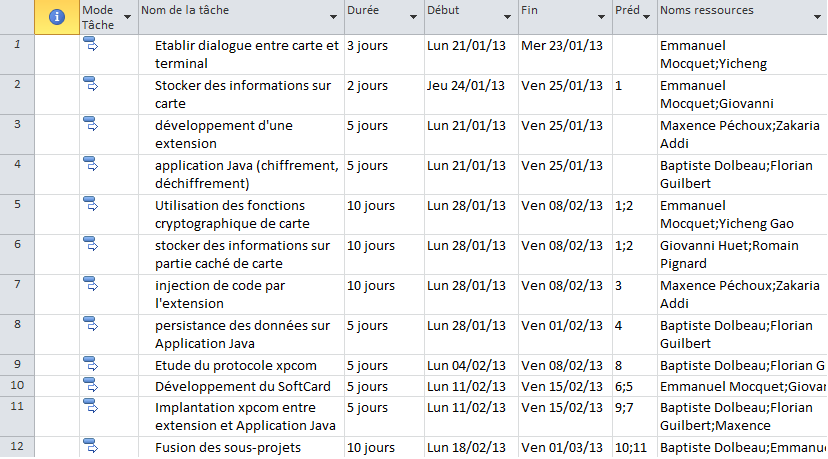
\includegraphics[scale=0.70]{ganttArray.png}
\caption{Diagramme de Gantt, tâches}
\end{figure}
% \newpage
\begin{figure}[!h]
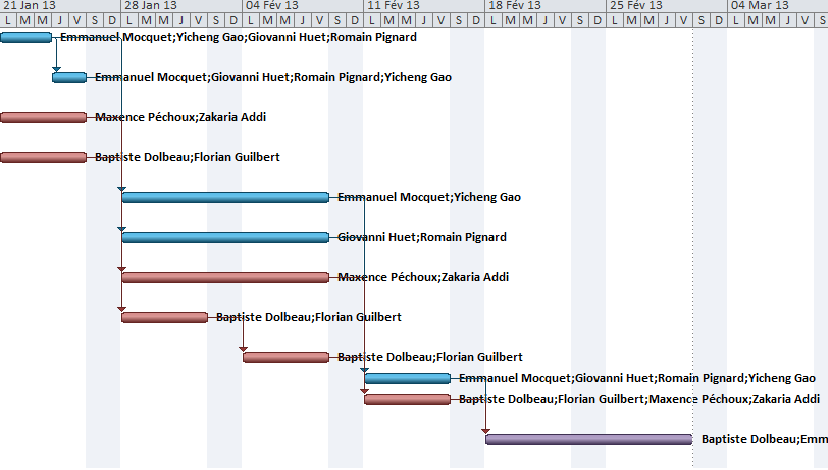
\includegraphics[scale=0.70]{ganttDiag.png}
\caption{Diagramme de Gantt, graphes}
\end{figure}
\end{center}
Sur ce graphe, on peut observer trois couleurs, le tâche bleue correspond
aux tâches correspondants au sous-projet \emph{smartCards}, le rouge aux
tâches du sous-projet \emph{Secure Social Network} et enfin le violet
correspond à la tâche fusion.
\section{Procédés de gestion}

\subsection{Gestion de la documentation}
Il y aura quatre documentations livrables : 
\begin{itemize}
 \item le manuel d'utilisation du \emph{softCard} rédigé par l'équipe testeur,
 du groupe \emph{smartCards};
 \item le manuel d'utilisation global de l'application rédigé par l'équipe 
 testeur, des deux groupes;
 \item un document décrivant comment ont été développées les applications pour
 la carte à puce et comment sont-elles installés;
 \item un document sur les protocoles cryptographiques mis en \oe{}uvre
 dans ce projet.
\end{itemize}
\paragraph{}
Les documents utilisées tout au long de la réalisation de ce projet sont : 
(les relecteurs sont encore à préciser)
\begin{itemize}
 \item Analyse des risques (AdR) rédigée par Yicheng \textsc{Gao};
 \item Cahier des recettes \emph{smartCard} (CdR) rédigé par Giovanni 
\textsc{Huet} et Romain \textsc{Pignard};
 \item Cahier des recettes \emph{Secure Social Network} (CdR) rédigé par 
 Baptiste \textsc{Dolbeau} et Florian \textsc{Guilbert};
 \item Document d'architecture logicielle \emph{smartCard} (DAL) rédigé par 
 Emmanuel \textsc{Mocquet};
 \item Document d'architecture logicielle \emph{Secure Social Network} (DAL) 
 rédigé par Zakaria \textsc{Addi} et Maxence \textsc{Péchoux};
 \item Plan de développement (PdD) rédigé par Florian \textsc{Guilbert};
 \item Spécification technique des besoins \emph{smartCard} (CdR) rédigée par 
 Giovanni \textsc{Huet} et Romain \textsc{Pignard};
 \item Spécification technique des besoins \emph{Secure Social Network} (CdR) 
    rédigée par Baptiste \textsc{Dolbeau} et Florian \textsc{Guilbert};
\end{itemize}

\subsection{Gestion des configurations}
Toutes les versions du programmes seront gérées par le logiciel de versionnage 
\texttt{git}. Toutes les machines servant à développer devront
avoir les même configurations du logiciel Java (1.5). De même, mais cela reste
à confirmer, les ordinateurs clients devront aussi posséder cette version de
Java.

\section{Revues et points clefs}
Pas de revues officielles de prévues.

\section{Procédures de suivi d'avancement}
Le suivi d'avancement du projet sera effectué par l'intermédiaire de réunions
régulières et de jalons. Ceux-ci permettront de contrôler l'état d'avancement
de chaque module et de réagir rapidement à tout écart avec les prévisions en
réorganisant le planning.

\paragraph{}
Il y aura par conséquent une réunion chaque semaine avec les clients respectifs
les membres du groupe. À chaque validation, il y aura présentation au client du 
travail effectué.

Des réunions avec le client pourront aussi être organisées si le client en fait
la demande ou bien qu'un membre du groupe souhaite bénéficier de son avis.

Pour chaque réunion, un compte-rendu sera réalisé et placé à disposition du
groupe par l'intermédiaire de \texttt{git}.

\end{document}
